%!TEX root = ../main.tex

\section{Experimental Results}
\label{sec:results}

%The output of our pipeline is two fold: the pose of the camera at each timestep and a mesh-based representation of the scene.
%To quantify the performance of the pose estimate we will be using both absolute and relative error metrics.
%These metrics will give us insights, respectively, on the global and local consistency of the trajectory estimate (\cref{ssec:state_estimation}).
%For the quality of the mesh we will be using a point cloud to point cloud distance as a metric to quantify how well the mesh represents the actual scene (\cref{ssec:mapping_quality}).
%We will also assess the real-time performance of the pipeline in \cref{ssec:timing}.
We benchmark the proposed approach against the state of the art on real datasets, and evaluate
 trajectory and map estimation accuracy, as well as runtime.
We use the \Euroc dataset~\cite{Burri15ijrr}, which contains visual and inertial data recorded from an micro aerial vehicle flying indoors.
The \Euroc dataset includes eleven datasets in total, recorded in two different scenarios.
The \textit{Machine Hall} scenario (\texttt{MH}) is the interior of an industrial facility.
It contains very little (planar) regularities.
The \textit{Vicon Room} (\texttt{V}) is similar to an office room where walls, floor and ceiling are close together, and other planar surfaces are visible
(boxes, stacked mattresses).
Datasets \texttt{V1} and \texttt{V2} differ only by the position of the objects in the scene.
%Moreover, each dataset is labelled by the level of difficulty it represents for Visual-Inertial SLAM algorithms: using the adjectives ``easy", ``medium", and ``difficult".
%The difficulty is increased by simply increasing the speed of the MAV, which results in motion-blur and drastic illumination changes on the images.
%For example, dataset \texttt{MH\_03\_medium} corresponds to a dataset in the Machine Hall where the MAV was flying at moderate speeds.
Each dataset provides the ground truth trajectory of the drone, allowing us to evaluate the accuracy of our estimation.
%compare our estimated trajectory with the real one.
For the \texttt{V} datasets, we are also provided with a ground truth point cloud of the scene, which we use to evaluate the accuracy of our mesh.

\mysubsection{Compared techniques}
To assess the advantages of our proposed approach, we compare three formulations that build one on top of the other.
First, we denote as \textbf{S}, the approach that would neither use regularity factors, nor projection factors, but only use Structureless factors ($\phi_{l_s}$, in \cref{eq:factor_form_c}).
Second, we denote as \textbf{SP}, the approach which would use Structureless factors, combined with Projection factors for those landmarks that have co-planarity constraints ($\phi_{l_c}$, in \cref{eq:factor_form_c}), but without using regularity factors.
Finally, we denote as \textbf{SPR}, our proposed formulation using Structureless, Projection and Regularity factors ($\phi_{\mathcal{R}}$, in \cref{eq:factor_form_a}).
The IMU factors ($\phi_{\text{IMU}}$, in \cref{eq:factor_form_b}) are implicitly used in all three formulations.
We also compare our results with other state-of-the-art implementations in \cref{tab:ape_accuracy_comparison_sopa}.
In particular, we compare the Root Mean Squared Error (RMSE) of our pipeline against OKVIS~\cite{Leutenegger13rss}, MSCKF~\cite{Mourikis07icra},
 ROVIO~\cite{Blosch15iros}, VINS-MONO~\cite{Qin17arxiv}, and SVO-GTSAM~\cite{Forster17troOnmanifold}, using the reported values in~\cite{Delmerico18benchmark}.
We refer the reader to \cite{Delmerico18benchmark} for details on the particular implementations and set of parameters used for each algorithm.
Note that these algorithms use a monocular camera, while we use a stereo camera.
Therefore, while \cite{Delmerico18benchmark} aligns the trajectories using $\mathrm{Sim}(3)$, we use instead $\mathrm{SE}(3)$.
Nevertheless, the scale is observable for all algorithms since they use an IMU.
We only report the values for VINS-MONO when its loop-closure module is disabled.

\subsection{Localization Performance}
\label{ssec:state_estimation}

%  One of the most important outputs of a VIO algorithm is an estimate of the
The state of our optimization problem comprises the poses of the IMU, the velocities, the IMU biases, the planes' parameters, and the landmarks' positions.
In this section we start by benchmarking the quality of the trajectory estimates, which are of paramount importance for control and AR/VR applications.
 The plane and landmark estimates will be assessed in the next \cref{ssec:mapping_quality}, where we evaluate the quality of the mesh.
We will assess the quality of the plane and landmark estimates in Section~\ref{ssec:mapping_quality}.

\mysubsection{Performance Metrics: Absolute Translation Error (ATE)}
\label{ssec:absolute_pose_error}
ATE looks at the translational part of the relative pose between the ground truth pose and the corresponding estimated pose at a given timestamp.
We first align our estimated trajectory with the ground truth trajectory both temporally and spatially (in SE(3)), as explained in \cite[Sec. 4.2.1]{RosinolMT}.
We refrain from using the rotational part since the trajectory alignment ignores the orientation of the pose estimates.
\Cref{tab:ape_all_datasets_pipelines} shows the ATE for our pipeline when using the pipelines S, SP, and our proposed approach SPR on the \Euroc dataset.

First, if we look at the performance of the different algorithmic variants for the datasets \texttt{MH\_03}, \texttt{MH\_04} and \texttt{MH\_05} in \cref{tab:ape_all_datasets_pipelines}, we observe that all methods perform equally.
This is because in these datasets no structural regularities were detected.
Hence, the proposed pipeline SPR gracefully downgrades to a standard structureless VIO pipeline (S).
Second, looking at the results
 for dataset \texttt{V2\_03}, we observe that both the SP and the SPR pipeline achieve the exact same performance.
In this case, structural regularities are detected, resulting in Projection factors being used.
Nevertheless, since the number of regularities detected is not sufficient to spawn a new plane estimate,
no structural regularities are actually enforced in the factor graph.
Finally, \cref{tab:ape_all_datasets_pipelines} shows that the SPR pipeline consistently achieves better results over the rest of datasets where structural regularities are detected and enforced.
In particular, the performance of SPR increases up to 28\% on the median ATE compared to the SP pipeline for datasets with multiple planes (e.g. \texttt{V1} and \texttt{V2}).

%We also divide the MAE by the length of the trajectory in order to be able to compare the performance between different datasets:
%\begin{equation}
  %\label{eq:ape_mae_percent}
  %\mathrm{Drift (\%)} = \frac{\frac{1}{N} \sum_{i=1}^N APE_i}{L},
%\end{equation}
%where $L$ is the length of the trajectory.

%\TODO{I still find this Drift misleading at best, at worst not representative of actual drift...
%We should be integrating the distance from start to point $i$ and dividing each $APE_i$ by this amount?}


\Cref{tab:ape_accuracy_comparison_sopa} shows that our approach, using structural regularities (SPR), achieves the best results when compared with the state-of-the-art,
 on datasets with structural regularities, such as in datasets \texttt{V1\_01\_easy} and \texttt{V1\_02\_medium},
  where multiple planes are present (walls, floor).
    We observe a $19\%$ improvement compared to the next best performing algorithm (SVO-GTSAM) in dataset \texttt{V1\_01\_easy},
     and a $26\%$ improvement in dataset \texttt{V1\_02\_medium} compared to ROVIO and VINS-MONO, which achieve the next best results.
    We also see that the performance of our pipeline is on-par with other state-of-the-art approaches when no structural regularities are present, such as in datasets \texttt{MH\_04\_difficult} and \texttt{MH\_05\_difficult}.

%\TODO{Important detail that I avoided altogether is that we are using the stereo camera also, while the above pipelines are all monocular. I just didn't mention stereo because then I have to add the stereo factors which make the whole story longer (Projection factors would now be mono/stereo etc).}
%Finally, we found to be instructive to color-code the estimated trajectory with the actual ATE errors at each pose estimate; which provides insights on how quickly the state estimation degrades.
%We provide these plots in the appendix of the thesis \TODO{cite Master's Thesis}.

% APE boxplots.
%\begin{figure*}[htbp]
  %\centering     %%% not \center
  %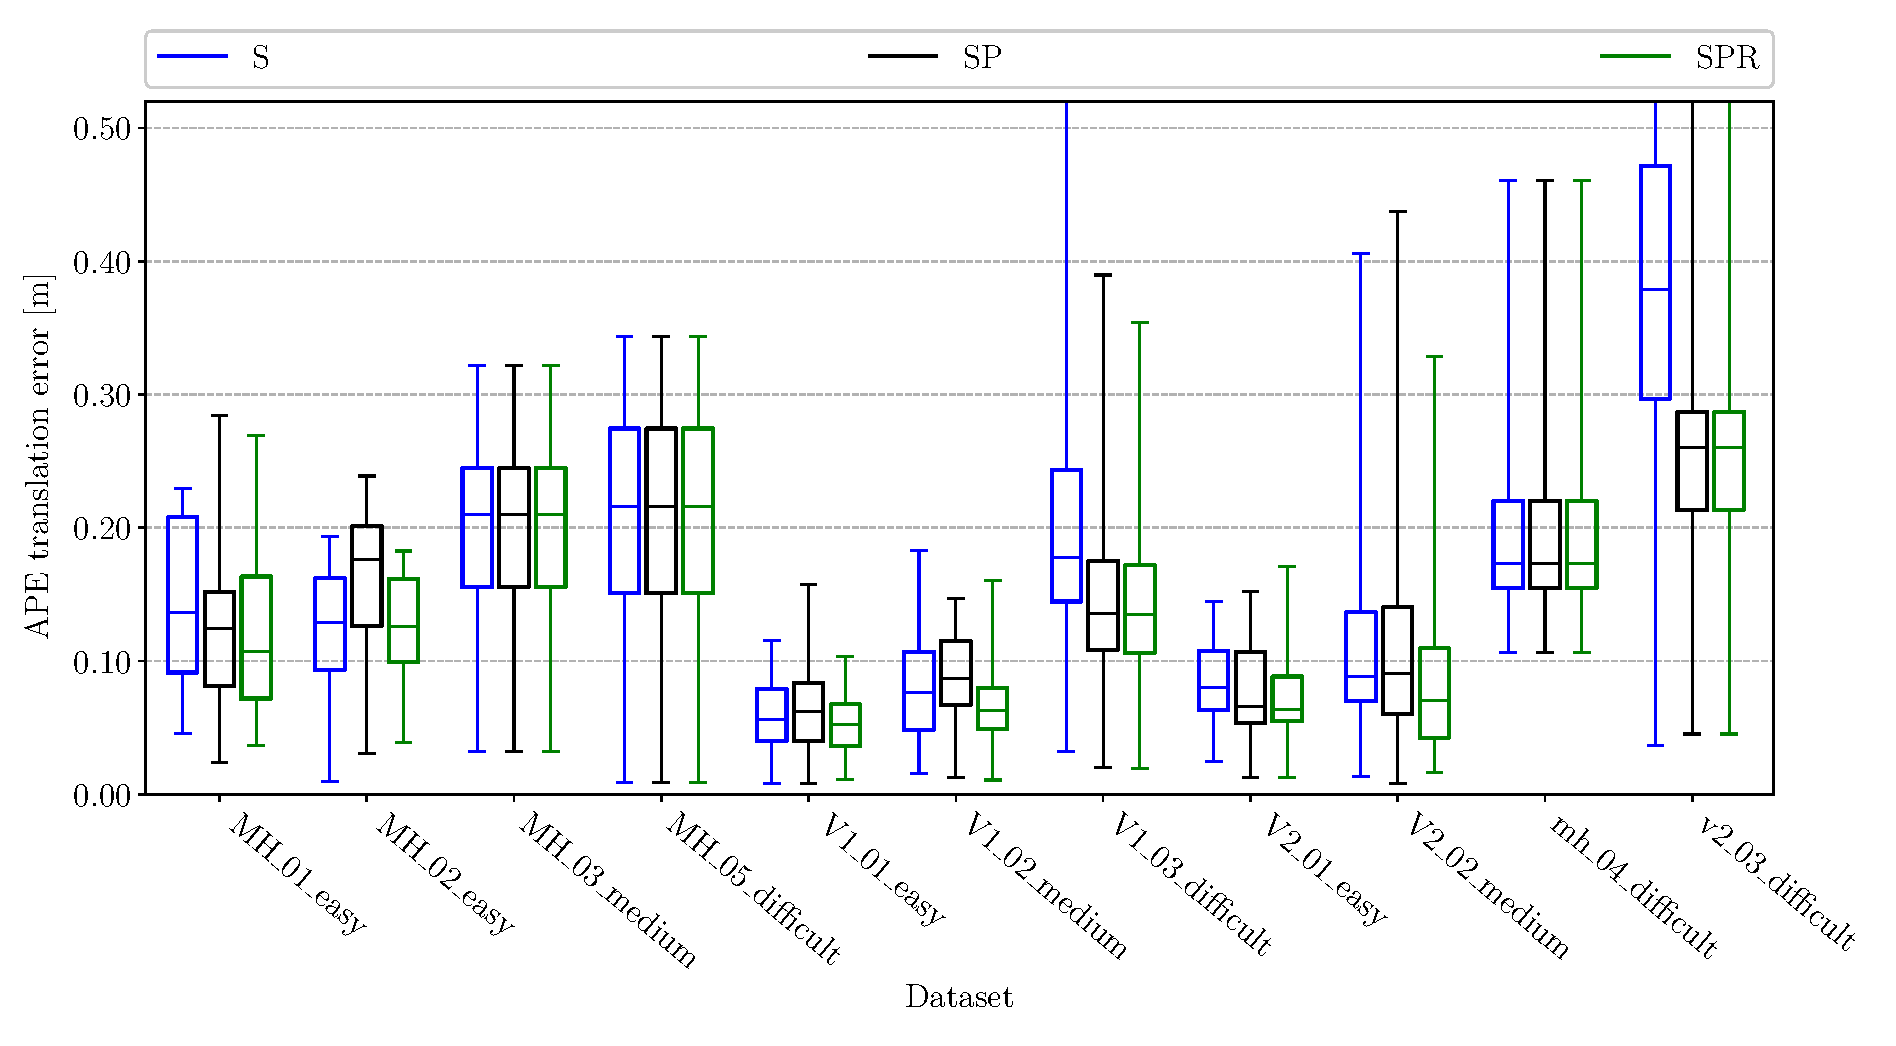
\includegraphics[trim={0 0 0 0cm},clip,width=0.7\textwidth]{datasets_ape_boxplots.eps}
  %\caption{Comparison of the Absolute Pose Error (APE) on the \Euroc{} datasets while using Structureless factors (S), Structureless and Projection factors (SP), and our proposed approach using Structureless, Projection and Regularity factors (SPR).}
  %\label{fig:ape_all_datasets_pipelines}
%\end{figure*}

% APE table results.
\begin{table}[tb]
  \centering
  \caption{ATE for pipelines S, SP, and SPR. Our proposed approach SPR achieves the best results for all datasets where structural regularities are detected and enforced.}
  \label{tab:ape_all_datasets_pipelines}
  \begin{tabularx}{\columnwidth}{l *6{Y}}
    \toprule
    & \multicolumn{6}{c}{ATE [cm]} \\
    \cmidrule{2-7}
    & \multicolumn{2}{c}{S} & \multicolumn{2}{c}{SP} & \multicolumn{2}{c}{SPR (\textbf{Proposed})} \\
    \cmidrule(r){2-3} \cmidrule(){4-5} \cmidrule(l){6-7}
    EuRoC Sequence & Median & RMSE & Median & RMSE & Median & RMSE \\
    \midrule
                 %MH\_01\_easy & 13.7 & 15.0 & 12.4 & 15.0 & \textbf{{10.7}} & \textbf{{14.5}} \\
             %MH\_02\_easy & 12.9 & 13.1 & 17.6 & 16.7 & \textbf{{12.6}} & \textbf{{13.0}} \\
           %MH\_03\_medium & 21.0 & 21.2 & 21.0 & 21.2 & 21.0 & 21.2 \\
        %MH\_04\_difficult & 17.3 & 21.7 & 17.3 & 21.7 & 17.3 & 21.7 \\
        %MH\_05\_difficult & 21.6 & 22.6 & 21.6 & 22.6 & 21.6 & 22.6 \\
             %V1\_01\_easy & 5.6 & 6.4 & 6.2 & 7.7 & \textbf{{5.3}} & \textbf{{5.7}} \\
           %V1\_02\_medium & 7.7 & 8.9 & 8.7 & 9.4 & \textbf{{6.3}} & \textbf{{7.4}} \\
        %V1\_03\_difficult & 17.7 & 23.1 & 13.6 & 17.6 & \textbf{{13.5}} & \textbf{{16.7}} \\
             %V2\_01\_easy & 8.0 & 8.9 & 6.6 & 8.2 & \textbf{{6.3}} & \textbf{{8.1}} \\
           %V2\_02\_medium & 8.8 & 12.7 & 9.1 & 13.5 & \textbf{{7.1}} & \textbf{{10.3}} \\
        %V2\_03\_difficult & 37.9 & 41.5 & 26.0 & 27.2 & 26.0 & 27.2 \\
                 %MH\_01\_easy & 13.7 & 15.0 & 12.4 & 15.0 & \textbf{{10.7}} & \textbf{{14.5}} \\

             MH\_02\_easy & 12.9 & 13.1 & 17.6 & 16.7 & \textbf{{12.6}} & \textbf{{13.0}} \\
             MH\_03\_medium & \textbf{21.0} & \textbf{21.2} & \textbf{21.0} & \textbf{21.2} &\textbf{21.0} & \textbf{21.2} \\
             MH\_04\_difficult & \textbf{17.3} & \textbf{21.7} & \textbf{17.3} & \textbf{21.7} & \textbf{17.3} &  \textbf{21.7} \\
             MH\_05\_difficult & \textbf{21.6} & \textbf{22.6} & \textbf{21.6} & \textbf{22.6} & \textbf{21.6} &  \textbf{22.6} \\
             V1\_01\_easy & 5.6 & 6.4 & 6.2 & 7.7 & \textbf{{5.3}} & \textbf{{5.7}} \\
           V1\_02\_medium & 7.7 & 8.9 & 8.7 & 9.4 & \textbf{{6.3}} & \textbf{{7.4}} \\
        V1\_03\_difficult & 17.7 & 23.1 & 13.6 & 17.6 & \textbf{{13.5}} & \textbf{{16.7}} \\
             V2\_01\_easy & 8.0 & 8.9 & 6.6 & 8.2 & \textbf{{6.3}} & \textbf{{8.1}} \\
           V2\_02\_medium & 8.8 & 12.7 & 9.1 & 13.5 & \textbf{{7.1}} & \textbf{{10.3}} \\
           V2\_03\_difficult & 37.9 & 41.5 & \textbf{26.0} & \textbf{27.2} & \textbf{26.0} & \textbf{27.2} \\
    \bottomrule
  \end{tabularx}%
\end{table}


% V1_01_easy
%\begin{figure}[htbp]
  %\centering

  %\begin{subfigure}[c]{0.7\columnwidth}
    %\resizebox{\columnwidth}{!}{\inputpgf{./results/V1_01_easy/SP/}{plots_APE_translation_trajectory_error.pgf}}
    %\subcaption{APE translation for S+P}
  %\end{subfigure}

  %\begin{subfigure}[c]{0.7\columnwidth}
    %\resizebox{\columnwidth}{!}{\inputpgf{./results/V1_01_easy/SPR/}{plots_APE_translation_trajectory_error.pgf}}
    %\subcaption{APE translation for S+PR}
  %\end{subfigure}

  %\caption{Dataset \texttt{V1\_01\_easy}: APE translation error plotted on the trajectory estimated by VIO using Strutureless and Projection factors (S + P), against our proposed approach using also Regularity factoris (S + P + R).}
  %\label{fig:ape_trans_traj_V1_01_easy}
%\end{figure}

%\begin{figure}[htbp]
  %\centering

  %\begin{subfigure}[c]{0.7\columnwidth}
    %\resizebox{\columnwidth}{!}{\inputpgf{./results/V1_01_easy/SP/}{plots_APE_translation.pgf}}
    %\subcaption{S+P}
  %\end{subfigure}

  %\begin{subfigure}[c]{0.7\columnwidth}
    %\resizebox{\columnwidth}{!}{\inputpgf{./results/V1_01_easy/SPR/}{plots_APE_translation.pgf}}
    %\subcaption{S+P+R}
  %\end{subfigure}

  %\caption{Dataset \texttt{V1\_01\_easy}: APE translation error of VIO using Strutureless and Projection factors (S + P), against our proposed approach using Structureless, Projection and Regularity factors (S +P + R).}
  %\label{fig:ape_trans_V1_01_easy}
%\end{figure}

% APE against state-of-the-art pipelines.

\begin{table}[tb]
  \centering
  \caption{ATE's RMSE of the state-of-the-art techniques (reported values from \cite{Delmerico18benchmark}) compared to our proposed SPR pipeline, on the \Euroc dataset. A cross ($\times$) states that the pipeline failed.
  In \textbf{bold} the best result, in \textcolor{blue}{blue} the second best.}
  \label{tab:ape_accuracy_comparison_sopa}
  \begin{tabularx}{\columnwidth}{l *6{Y}}
    \toprule
    & \multicolumn{6}{c}{RMSE ATE [cm]} \\
    \cmidrule(l){2-7}
    Sequence  & OKVIS & MSCKF & ROVIO & VINS-MONO & SVO-GTSAM & \textbf{SPR} \\
    \midrule
    MH\_01\_e & 16 & 42 & 21 & 27 & \textbf{5} & \textbf{\textcolor{blue}{14}} \\
    MH\_02\_e & 22 & 45 & 25 & \textbf{\textcolor{blue}{12}} & \textbf{3} & 13 \\
    MH\_03\_m & 24 & 23 & 25 & \textbf{\textcolor{blue}{13}} & \textbf{12} & 21 \\
    MH\_04\_d & 34 & 37 & 49 & 23 & \textbf{13} & \textbf{\textcolor{blue}{22}} \\
    MH\_05\_d & 47 & 48 & 52 & 35 & \textbf{16} & \textbf{\textcolor{blue}{23}} \\
    V1\_01\_e & 9 & 34 & 10 & \textbf{\textcolor{blue}{7}} & \textbf{\textcolor{blue}{7}} & \textbf{6} \\
    V1\_02\_m & 20 & 20 & \textbf{\textcolor{blue}{10}} & \textbf{\textcolor{blue}{10}} & 11 & \textbf{7} \\
    V1\_03\_d & 24 & 67 & \textbf{\textcolor{blue}{14}} & \textbf{13} & $\times$ & 17 \\
    V2\_01\_e & 13 & 10 & 12 & \textbf{\textcolor{blue}{8}} & \textbf{7} & \textbf{\textcolor{blue}{8}} \\
    V2\_02\_m & 16 & 16 & 14 & \textbf{8} & $\times$ & \textbf{\textcolor{blue}{10}} \\
    V2\_03\_d & 29 & 113 & \textbf{14} & \textbf{\textcolor{blue}{21}} & $\times$ & 27 \\
    \bottomrule
  \end{tabularx}%
\end{table}


    %MH\_01\_e & 16 & 42 & 21 & 27 & \textbf{5} & 14.5 \\
    %MH\_02\_e & 22 & 45 & 25 & 12 & \textbf{3} & 13.0 \\
    %MH\_03\_m & 24 & 23 & 25 & 13 & \textbf{12} & 21.2 \\
    %MH\_04\_d & 34 & 37 & 49 & 23 & \textbf{13} & 21.7 \\
    %MH\_05\_d & 47 & 48 & 52 & 35 & \textbf{16} & 22.6 \\
    %V1\_01\_e & 9 & 34 & 10 & 7 & 7 & \textbf{5.7} \\
    %V1\_02\_m & 20 & 20 & 10 & 10 & 11 & \textbf{7.4} \\
    %V1\_03\_d & 24 & 67 & 14 & \textbf{13} & $\times$ & 16.7 \\
    %V2\_01\_e & 13 & 10 & 12 & 8 & \textbf{7} & 8.1 \\
    %V2\_02\_m & 16 & 16 & 14 & \textbf{8} & $\times$ & 10.3 \\
    %V2\_03\_d & 29 & 113 & \textbf{14} & 21 & $\times$ & 27.2 \\

%\TODO{Say that in datasets where there are no structural regularities we are actually comparing our non-regular pipeline implementation against the others... but ours has not been optimized...}

\mysubsection{Performance Metrics: Relative Pose Error (RPE)}
\label{ssec:relative_pose_error}
While the ATE provides information on the global consistency of the trajectory estimate, it does not provide insights on the moment in time when the erroneous estimates happen.
Instead, the Relative Pose Error (RPE) is a metric for investigating the local consistency of a SLAM trajectory.
RPE aligns the estimated and ground truth pose for a given frame $i$, and then computes the error of the estimated pose for a frame $j>i$ at a fixed distance farther along the trajectory.
We calculate the RPE from frame $i$ to $j$ in translation and rotation (absolute angular error) \cite[Sec. 4.2.3]{RosinolMT}.
As \cite{Geiger12cvpr}, we evaluate the RPE over all possible trajectories of a given length, and for different lengths.
Nevertheless, instead of calculating the mean of all RPE for a given trajectory length, we report the maximum, the minimum, the first and third quartile, as well as the median.

\mysubsection{RPE results}
In \Cref{fig:boxplot_rpe}, we show the results for dataset \texttt{V2\_02}, where we observe that using our proposed pipeline SPR, with respect to the SP pipeline, leads to: (i) an accuracy improvement of up to 50\% in translation and 30\% in rotation (based on the maximum improvement on the median of the errors), and, (ii) an average improvement over all trajectory lenghts of 20\% in translation and 15\% in rotation (for the median errors).

%\begin{figure}[htbp]
  %\centering     %%% not \center

  %\begin{subfigure}[c]{0.7\columnwidth}
    %\includegraphics[trim={0 0 0 0cm},clip,width=\columnwidth]{./results/MH_03_medium/traj_relative_errors_boxplots.eps}
    %\subcaption{\texttt{MH\_03\_medium}}
    %\label{fig:boxplot_rpe_mh_03_v2_03_subfig_a}
  %\end{subfigure}
  %\begin{subfigure}[c]{0.7\columnwidth}
    %\includegraphics[trim={0 0 0 0cm},clip,width=\columnwidth]{./results/v2_03_difficult/traj_relative_errors_boxplots.eps}
    %\subcaption{\texttt{V2\_03\_difficult}}
    %\label{fig:boxplot_rpe_mh_03_v2_03_subfig_b}
  %\end{subfigure}

  %\caption{Detailed comparison of the state estimation accuracy while using Structureless factors (S), Structureless and Projection factors (SP), and our proposed approach using Structureless, Projection and Regularity factors (SPR) on \Euroc{}'s V1\_02\_medium and V2\_02\_medium datasets.}

  %\label{fig:boxplot_rpe_mh_03_v2_03}
%\end{figure}

\begin{figure}[htbp]
  \centering     %%% not \center

    %\includegraphics[trim={0 13.5cm 0 0cm},clip,width=0.5\columnwidth]{./results/V1_02_medium/traj_relative_errors_boxplots.eps}
    %\includegraphics[trim={0.1cm 0 0.05cm 1.25cm},clip,width=0.52\columnwidth]{./results/V1_02_medium/traj_relative_errors_boxplots.eps}
    %\hspace{-1em}
    %\includegraphics[trim={1.0cm 0 0.2cm 1.25cm},clip,width=0.4605\columnwidth]{./results/V2_02_medium/traj_relative_errors_boxplots.eps}
    %\includegraphics[trim={0cm 0 0cm 0cm},clip,width=\columnwidth]{./results/V1_02_medium/traj_relative_errors_boxplots.eps}
    \includegraphics[trim={0.1cm 0 0cm 0.2cm},clip,width=0.8\columnwidth]{./results/V2_02_medium/traj_relative_errors_boxplots.eps}

  \caption{Detailed comparison of the state estimation accuracy while using pipeline S, SP, and our proposed approach SPR on different \Euroc{} datasets.}

  \label{fig:boxplot_rpe}
\end{figure}

\subsection{Mapping quality}
\label{ssec:mapping_quality}
We use the ground truth point cloud for \texttt{V1} dataset to assess the quality of the mesh by calculating its \textit{accuracy} as defined in \cite{Schoeps2017cvpr}.

\mysubsection{Performance Metric: Map Accuracy}
  \label{ssec:map_accuracy}
%   by calculating its \textit{accuracy} %(\cref{ssec:map_accuracy})
% as defined in \cite{Schoeps2017cvpr}.
Comparing a mesh with a dense point cloud can be achieved by generating a point cloud from the mesh itself, and then comparing both point clouds.
In our case, we compute a point cloud by sampling the mesh with a uniform density of $10^3$ points per square meter.
We also register the resulting point cloud to the ground truth point cloud using an iterative closest point algorithm.
%
%\TODO{Here we are not saying how we merge sparse meshes together for evaluation (we are not just appending time-horizon meshes together...)}
  With the newly registered point cloud, we can compute a cloud to cloud distance to assess the accuracy of the mesh relative to the ground truth point cloud.
  More specifically, for each point $r$ of the estimated cloud from the mesh $\mathcal{R}$, we search the nearest point in the ground truth cloud $\mathcal{G}$, and compute their Euclidean distance $d_{r \to \mathcal{G}}$:

  \begin{equation}
    \label{eq:c2c_distance}
    d_{r \to \mathcal{G}} = \min_{g \in \mathcal{G}}\left\|{r-g}\right\|_{2} \quad\text{for}\quad r \in \mathcal{R}.
  \end{equation}

  \Cref{tab:mesh_accuracy_stats_comparison} shows that both the mean and the standard deviation of the distance from the mesh to the ground truth point cloud (\cref{eq:c2c_distance}) decreases when enforcing structural regularities, as done in the SPR pipeline.
  On average, each point sampled on the mesh generated by the SPR pipeline is $0.5$ cm closer to the ground truth point cloud than the points sampled on the mesh generated by the SP pipeline.
  Therefore, enforcing structural regularities makes the estimated mesh closer to the real scene.

  We also report the accuracy $\mathcal{A}(\tau)$, defined as the fraction of estimated points which are within a distance threshold $\tau$ of the ground truth point cloud \cite{Schoeps2017cvpr, Knapitsch2017}:
  \begin{equation}
    \label{eq:mesh_accuracy}
    \mathcal{A}(\tau) = \frac{1}{|\mathcal{R}|}\sum_{r \in \mathcal{R}}\bigg[d_{r \to \mathcal{G}} < \tau\bigg]_I \times 100,
  \end{equation}
  where $[P]_I$ is the Iverson bracket, defined as:
  \begin{equation*}
    [P]_I={\begin{cases}
        1&{\text{if }}P{\text{ is true;}}\\
        0&{\text{otherwise,}}
    \end{cases}}
  \end{equation*}

  \Cref{fig:histogram_accuracy_mesh} shows the actual error distributions for $d_{r \to \mathcal{G}}$, and the mesh accuracy $\mathcal{A}(\tau)$ for different distance thresholds $\tau$, for both the SP and the SPR pipelines respectively.
  In terms of accuracy values $\mathcal{A}(\tau)$, we can see in \cref{fig:histogram_accuracy_mesh} that the SPR pipeline consistently achieves more accurate mesh estimates (between 3\%-7\% better) for distance thresholds $\tau < 10cm$.

  As a reminder, the SP pipeline still uses the mesh to detect regularities, but, contrary to the SPR pipeline, it does not enforce the structural regularities on the landmarks.

  In \cref{fig:accuracy_mesh}, we color-encode each point on the estimated point cloud with the error distances $d_{r \to \mathcal{G}}$.
  We can observe that, when we do not enforce structural regularities, significant errors are actually present on the planar surfaces, especially on the walls (\cref{fig:accuracy_mesh} top).
  Instead, when regularities are enforced, the errors on the walls and the floor are reduced (\cref{fig:accuracy_mesh} bottom).
\TODO{Remove everything except this and the results in table 3}  A closer view on the wall itself, bottom figures (c) and (d) of \cref{fig:intro}, shows that it is visually clear that adding co-planarity constraints results in smoother walls.

% Cloud comparison table
\begin{table}[]
  \caption{Statistics for the cloud to cloud absolute distance from the mesh to the ground truth point cloud $d_{r \to \mathcal{G}}$ (\cref{eq:c2c_distance}) for dataset \texttt{V1\_01\_easy}.}
  \label{tab:mesh_accuracy_stats_comparison}
  \centering
  \begin{tabularx}{\columnwidth}{l *2{Y}}%
    \toprule
    & \multicolumn{2}{c}{VIO Type} \\
    \cmidrule(lr){2-3}
    $d_{r \to \mathcal{G}}$ Statistics & SP & SPR (\textbf{Proposed}) \\
    \cmidrule(lr){2-2} \cmidrule(lr){3-3}
    Mean $\bar{d}_{\mathcal{R}}$ [cm] & 4.9 & \textbf{4.4} \\
    Standard Deviation $\sigma_{\mathcal{R}}$ [cm] & 5.0 & \textbf{4.6} \\
    \bottomrule
  \end{tabularx}
\end{table}

% ground truth point cloud.
%\begin{figure}[tb]
%  \centering     %%% not \center
%  \includegraphics[trim={0 0 0 0cm},clip,height=0.5\columnwidth, width=\columnwidth]{./results/gt_point_cloud/V1_01_easy/frames_animation/frame_000000.png}
%  \caption{ground truth point cloud. Color-encoded for better visualization.}
%  \label{fig:ground_truth_point_cloud}
%\end{figure}

% Mesh accuracy histograms
\begin{figure}[tb]
  \centering     %%% not \center
  %\adjustbox{width=\columnwidth,trim=0.0cm 0pt 0.2ex 0pt,clip}{\resizebox{0.49\textwidth}{!}{\inputpgf{./results/S_P_Mesh/Histogram/}{Histogram_for_paper_accuracy_S_P.pgf}}}
  \adjustbox{width=\columnwidth,trim=0.1cm 0 0.1cm 0,clip}{\resizebox{\columnwidth}{!}{\inputpgf{./results/S_P_R_Mesh/Histogram/}{Histogram_for_paper_accuracy_S_P_R.pgf}}}

  %\caption{(Top) Histogram of points sampled on the mesh depending on their distance to the ground truth point cloud ($d_{r \to \mathcal{G}}$) for dataset \texttt{V1\_01\_easy} and pipelines SP (left) and SPR (right).
  %Detailed is the mesh accuracy $\mathcal{A}(\tau)$, as defined in \cref{eq:mesh_accuracy}, for different distance thresholds $\tau$. (Bottom) Color-encoded point cloud sampled from the estimated 3D mesh. The colormap is the same for all figures.}
  \caption{Histogram of points sampled on the mesh depending on their distance to the ground truth point cloud ($d_{r \to \mathcal{G}}$) for dataset \texttt{V1\_01\_easy} and pipelines SP (left) and SPR (right).
  Detailed is the mesh accuracy $\mathcal{A}(\tau)$, as defined in \cref{eq:mesh_accuracy}, for different distance thresholds $\tau$.}
  \label{fig:histogram_accuracy_mesh}
\end{figure}

\subsection{Timing}
\label{ssec:timing}

The pipelines S, SP, and SPR differ in that they try to solve an increasingly complicated problem.
While the S pipeline does not include neither the 3D landmarks nor the planes as variables in the optimization problem, the SP pipeline includes 3D landmarks, and the pipeline using regularities (SPR) further includes planes as variables.
Moreover, the SP has significantly less constraints between the variables than the SPR pipeline.
Hence, we can expect that the optimization times for the different pipelines will be each bounded by the other as $t_{S}^{opt} < t_{SP}^{opt} < t_{SPR}^{opt}$, where $t_{X}^{opt}$ is the time taken to solve the optimization problem of pipeline X.

\Cref{fig:optimization_time} shows the time taken to solve the optimization problem for each type of pipeline.
Experimentally, we observe that the optimization time follows roughly the expected distribution $t_{S}^{opt} < t_{SP}^{opt} < t_{SPR}^{opt}$.
We also observe that if the number of plane variables is large ($\sim 10^1$), and consequently the number of constraints between landmarks and planes also gets large ($\sim 10^2$), the optimization problem cannot be solved in real-time.
For example, for the keyframe index 250 in \Cref{fig:optimization_time}, we can see that a spike is present caused by the detection of multiple planes and landmarks with regularities.

\begin{figure}[tb]
  \centering     %%% not \center
    \resizebox{\columnwidth}{!}{\inputpgf{./img/}{all_timing_for_paper.pgf}}
  \caption{Comparison of the time to solve the optimization problem for pipeline S, SP, and SPR for dataset \texttt{V1\_01\_easy}.}
  \label{fig:optimization_time}
\end{figure}



